%% QIT_paper.tex — Quantum Interference Transformer
%% Build: make  (or: pdflatex QIT_paper && bibtex QIT_paper && pdflatex QIT_paper && pdflatex QIT_paper)

\documentclass[11pt,a4paper]{article}

%% ── Encoding & fonts ─────────────────────────────────────────────────────────
\usepackage[T1]{fontenc}
\usepackage[utf8]{inputenc}
\usepackage{lmodern}
\usepackage{microtype}

%% ── Page layout ──────────────────────────────────────────────────────────────
\usepackage[top=1in,bottom=1in,left=1.2in,right=1.2in]{geometry}
\setlength{\parskip}{0.4em}
\setlength{\parindent}{0pt}

%% ── Math ─────────────────────────────────────────────────────────────────────
\usepackage{amsmath}
\usepackage{amssymb}
\usepackage{amsthm}
\usepackage{bm}

%% ── Graphics ─────────────────────────────────────────────────────────────────
\usepackage{graphicx}
\usepackage[dvipsnames,table]{xcolor}

%% ── Tables ───────────────────────────────────────────────────────────────────
\usepackage{booktabs}
\usepackage{array}
\newcolumntype{L}[1]{>{\raggedright\arraybackslash}p{#1}}
\newcolumntype{C}[1]{>{\centering\arraybackslash}p{#1}}
\newcolumntype{R}[1]{>{\raggedleft\arraybackslash}p{#1}}

%% ── Code listings ────────────────────────────────────────────────────────────
\usepackage{listings}
\lstset{
    basicstyle   = \ttfamily\small,
    breaklines   = true,
    frame        = single,
    rulecolor    = \color{gray!40},
    backgroundcolor = \color{gray!5},
    keywordstyle = \color{blue!70!black}\bfseries,
    commentstyle = \color{gray}\itshape,
    stringstyle  = \color{orange!80!black},
    numbers      = none,
    xleftmargin  = 4pt,
    xrightmargin = 4pt,
}

%% ── Section spacing ──────────────────────────────────────────────────────────
\makeatletter
\renewcommand\section{\@startsection{section}{1}{\z@}%
  {1.4ex \@plus 0.4ex}{0.6ex}{\normalfont\large\bfseries}}
\renewcommand\subsection{\@startsection{subsection}{2}{\z@}%
  {1.1ex \@plus 0.3ex}{0.4ex}{\normalfont\normalsize\bfseries}}
\renewcommand\subsubsection{\@startsection{subsubsection}{3}{\z@}%
  {0.9ex \@plus 0.2ex}{0.3ex}{\normalfont\normalsize\bfseries}}
\makeatother

%% ── References & hyperlinks ──────────────────────────────────────────────────
\usepackage[numbers,sort&compress]{natbib}
\usepackage[colorlinks=true,
            linkcolor=blue!65!black,
            citecolor=green!45!black,
            urlcolor=blue!65!black]{hyperref}

%% ── Custom macros ────────────────────────────────────────────────────────────
\newcommand{\ket}[1]{|{#1}\rangle}
\newcommand{\bra}[1]{\langle{#1}|}
\newcommand{\expected}[1]{\langle{#1}\rangle}
\newcommand{\Uenc}{U_{\!\text{encode}}}
\newcommand{\Uent}{U_{\!\text{entangle}}}
\newcommand{\Uatt}{U_{\!\text{attention}}}
\newcommand{\Umix}{U_{\!\text{mix}}}
\newcommand{\UQIT}{U_{\!\text{QIT}}}
\newcommand{\planned}{\textcolor{gray!70!black}{\textbf{[Planned]}}}
\newcommand{\Ftwo}{\mathbb{F}_2}

%% ── Abstract style ───────────────────────────────────────────────────────────
\renewenvironment{abstract}{%
  \small\begin{center}\textbf{Abstract}\end{center}%
  \begin{quotation}\noindent}{\end{quotation}}

%% ─────────────────────────────────────────────────────────────────────────────
\begin{document}

\title{\textbf{Quantum Interference Transformer (QIT):\\
       Emergent Sequence Intelligence from Amplitude Dynamics}}

\author{Mihail Stancescu\\[2pt]
        \small Independent Research\\
        \small \href{mailto:madmishu007@gmail.com}{madmishu007@gmail.com}}

\date{Draft v0.1 \quad \today \quad \textit{Working paper / preprint}}

\maketitle
\thispagestyle{empty}

%% ── Abstract ─────────────────────────────────────────────────────────────────
\begin{abstract}
We introduce the \textbf{Quantum Interference Transformer} (QIT), a sequence model
in which token relationships are resolved not by dot-product attention scores, but by
constructive and destructive interference within a parameterised quantum circuit.
The central claim is modest but concrete: \emph{sequence intelligence can emerge from
interference dynamics}, and an interference-based attention mechanism is measurably
more sample-efficient than classical attention on structured tasks that have a natural
phase-kickback representation.

We present \textbf{QIT-0}, a minimal prototype built on PennyLane~\cite{bergholm2018pennylane}
and PyTorch. The architecture encodes a token sequence into qubit rotation angles,
seeds cross-token correlations via a ring CNOT ladder, applies a learned
strongly-entangling unitary as the attention operator, and reads out Pauli-$Z$
expectation values as the hidden state. A single linear layer decodes these to class logits.

On the 4-bit binary parity task --- a memorisation benchmark over all 16 inputs ---
QIT-0 (78~parameters) reaches 100\% accuracy in \textbf{6.2\,$\pm$\,1.7 epochs}
(mean\,$\pm$\,std over 5 random seeds, all 5 converging).
An MLP (94~parameters) requires 31.7\,$\pm$\,4.1~epochs (3\,/\,5 seeds converge in 200~epochs),
a GRU (110~parameters) requires 34.5\,$\pm$\,5.5~epochs (2\,/\,5 converge),
and a classical Transformer~\cite{vaswani2017attention} (206~parameters) fails to converge
in 200~epochs under any of the 5 seeds tested.
A logistic regression baseline on the sum-feature representation
$f(\mathbf{x}) = \sum_i x_i$ also fails to converge --- parity is not linearly separable
even with this structural feature, as the decision boundary is non-monotone in the sum.
Wall-clock time per epoch is $\approx$195~ms due to quantum simulation overhead,
compared to sub-2~ms for classical models; this cost is intrinsic to software simulation
and is not representative of future hardware execution.

We do not claim that quantum computation is generally superior to classical computation
for machine learning. We claim that for tasks whose structure maps naturally to quantum
phase dynamics, interference-based attention exhibits strong inductive bias and
superior sample efficiency.
\end{abstract}

\vspace{1em}
\hrule
\vspace{1em}

%% ── Table of Contents (optional for draft) ───────────────────────────────────
\tableofcontents
\newpage

%% ─────────────────────────────────────────────────────────────────────────────
\section{Introduction}
\label{sec:intro}

The dominant paradigm for sequence modelling is softmax attention~\cite{vaswani2017attention},
in which relevance between token pairs is computed as an explicit dot-product similarity
followed by a normalised weighted sum of values. This mechanism is expressive and
well-understood, but it imposes a particular inductive bias: relevance is a scalar
pairwise comparison, and aggregation is a convex combination. Whether this is the
\emph{only} useful inductive bias for sequence tasks is an open question.

Quantum mechanics offers an alternative picture of how information from multiple sources
can be combined. In quantum circuits, information propagates as complex amplitudes, and
multiple signal paths interfere. Paths with aligned phases amplify each other
(\emph{constructive} interference); paths with opposing phases cancel
(\emph{destructive} interference). The result of a computation is determined not by
explicit similarity scoring but by the global amplitude pattern that emerges from the
circuit geometry and the learned unitary parameters. Critically, this mechanism is
\emph{non-local by construction}: a single layer of entangling gates connects every
qubit to every other, giving the circuit access to all token positions simultaneously.

This paper asks a simple question: \emph{can this interference dynamic serve as a
drop-in replacement for dot-product attention?}

To answer it, we build QIT-0, the first prototype of the Quantum Interference
Transformer. QIT-0 is explicitly a proof-of-concept, not a production system. The
circuit runs on a classical quantum simulator (PennyLane's \texttt{default.qubit}),
which makes wall-clock time uncompetitive with classical models. The vocabulary is binary
(2~tokens), the sequence length is 4, and the only task is parity. But the results are
striking: the interference mechanism finds the parity function in 12.4 gradient steps (mean, 5~seeds),
while the classical Transformer with 2.6$\times$ more parameters fails to converge
in 400 gradient steps (200~epochs) across all seeds tested.

The paper is organised as follows. Section~\ref{sec:background} reviews the relevant
background. Section~\ref{sec:architecture} describes the QIT architecture in full.
Section~\ref{sec:experiments} describes the experimental setup. Section~\ref{sec:results}
presents results. Section~\ref{sec:discussion} discusses what the results mean and what
they do not mean. Section~\ref{sec:future} describes planned future work.
Section~\ref{sec:conclusion} concludes.

%% ─────────────────────────────────────────────────────────────────────────────
\section{Background}
\label{sec:background}

\subsection{Classical Attention}

The scaled dot-product attention mechanism introduced by Vaswani et al.~\cite{vaswani2017attention}
computes, for a sequence of token representations $X \in \mathbb{R}^{n \times d}$:

\begin{equation}
  \text{Attention}(Q, K, V)
    = \text{softmax}\!\left(\frac{QK^\top}{\sqrt{d_k}}\right) V
  \label{eq:attention}
\end{equation}

where $Q = XW_Q$, $K = XW_K$, $V = XW_V$ are learned linear projections.
The softmax produces a probability distribution over positions, used to form a weighted
sum of value vectors. Relevance between tokens is an explicit bilinear function of
their representations.

This mechanism is powerful but has several well-known properties. The quadratic cost in
sequence length $O(n^2 d)$ limits scalability. The inductive bias --- similarity as a
dot product --- is appropriate for many tasks but is not a universal prior. Even a minimal
single-head Transformer for 4-token binary sequences requires 206~parameters in our experiments.

\subsection{Quantum Computing Fundamentals}

A quantum system of $n$ qubits exists in a superposition over $2^n$ computational basis
states. The state is described by a complex amplitude vector
$\ket{\psi} \in \mathbb{C}^{2^n}$ with $\|\ket{\psi}\|^2 = 1$. Evolution is governed by
unitary operators $U$; measurement in the computational basis collapses the state and
yields classical outcomes with probabilities determined by the squared amplitudes.

The Pauli-$Z$ expectation value for qubit $i$ is:
\begin{equation}
  \expected{Z_i} = \bra{\psi} Z_i \ket{\psi} \in [-1,\,1]
  \label{eq:expval}
\end{equation}

This provides a real-valued readout differentiable with respect to circuit parameters via
the parameter-shift rule~\cite{schuld2019evaluating}, enabling gradient-based training.

\textbf{Angle encoding} maps a real value $x$ to the rotation
$RY(x) = e^{-i x \sigma_y / 2}$, where $\sigma_y$ is the Pauli-$Y$ operator.
For inputs in $[-\pi, \pi]$, this sweeps the full Bloch sphere. The encoded state is:
\begin{equation}
  \ket{\phi(x)} = \cos\!\left(\tfrac{x}{2}\right)\ket{0} + \sin\!\left(\tfrac{x}{2}\right)\ket{1}
  \label{eq:angle_enc}
\end{equation}

\textbf{Entanglement} is the key non-classical resource. A CNOT gate on wires $(c, t)$
maps $\ket{c, t} \mapsto \ket{c,\; c \oplus t}$, creating correlations between previously
independent qubits. Once entangled, the state cannot be described as a product of
independent qubit states: information is genuinely distributed across the register.

\textbf{Interference} is the mechanism by which quantum circuits compute. A
parameterised unitary $U(\theta)$ steers amplitudes: for inputs mapping to the same
output, amplitude paths constructively interfere and expectation values are amplified;
for inputs mapping to different outputs, amplitudes destructively interfere and are
suppressed.

\subsection{Quantum Machine Learning Context}

Variational quantum circuits (VQCs) as machine learning models have been studied
extensively since Farhi \& Neven~\cite{farhi2018classification} and
Mitarai et al.~\cite{mitarai2018quantum}. Benedetti et al.~\cite{benedetti2019parameterized}
provide a systematic treatment of parameterised circuits as learning models;
Cerezo et al.~\cite{cerezo2021variational} and Biamonte et al.~\cite{biamonte2017quantum}
offer broader surveys. A critical trainability concern for deep VQCs is the \emph{barren
plateau} phenomenon~\cite{mcclean2018barren}: gradient variance can decay exponentially
with qubit count, making training intractable at scale. We verify that QIT-0 at $n=8$
qubits does not exhibit this pathology (see \S\ref{sec:gradvar}).

\textbf{Quantum kernel theory.} Havl\'{i}\v{c}ek et al.~\cite{havlicek2019supervised}
demonstrate that angle-encoded quantum circuits implicitly compute a kernel function
$k(\mathbf{x}, \mathbf{x}') = |\langle \Psi(\mathbf{x}) | \Psi(\mathbf{x}') \rangle|^2$
over quantum feature space. Schuld~\cite{schuld2021kernel} formalises this: any VQC
classifier is equivalent to a kernel method with the circuit's feature map as the kernel.
This framework directly applies to QIT. The angle encoding + entanglement layer defines
a quantum feature map; the parity advantage can be understood as this kernel being better
aligned with the parity decision boundary than any classical polynomial kernel of
comparable parameter count. Abbas et al.~\cite{abbas2021power} characterise the
effective dimension of quantum neural networks and show that certain circuit architectures
can achieve higher Fisher information per parameter than classical alternatives.

\textbf{Quantum natural language processing.} Lorenz et al.~\cite{lorenz2023qnlp}
demonstrate compositional quantum language models running on real quantum hardware,
establishing that quantum sequence processing is operationally feasible beyond simulators.
QIT targets a different regime (interference as attention rather than compositional
structure), but the QNLP programme establishes that quantum sequence models are a
coherent research direction.

\textbf{Relation to quantum attention proposals.} The idea of replacing classical attention
with a quantum subroutine is nascent. Prior proposals have considered inner-product
similarity computed in Hilbert space, quantum kernel methods for attention scoring, and
amplitude-based retrieval analogous to associative memory. QIT differs from these in a
key respect: we do not attempt to accelerate or quantise the classical dot-product attention
computation. Instead, we replace the attention \emph{concept} --- explicit pairwise scoring ---
with interference \emph{dynamics}, in which token relationships emerge from the global
amplitude pattern produced by an entangling unitary. This is a fundamentally different
inductive bias, not a speed-up of an existing one.

Bowles et al.~\cite{bowles2024benchmarking} raise important methodological cautions
about QML benchmarks: classical simulation overhead, cherry-picked tasks, and lack of
statistical rigour are common pitfalls. We address these directly: results are reported
over multiple seeds, we include a negative-control task (first-token detection,
\S\ref{sec:firsttoken}), and wall-clock costs are reported honestly.

%% ─────────────────────────────────────────────────────────────────────────────
\section{QIT Architecture}
\label{sec:architecture}

\subsection{Overview}

The full QIT-0 pipeline (Figure~\ref{fig:pipeline}) is composed of three sequential
components: a classical embedding, the quantum interference attention block (\S\ref{sec:qia}),
and a classical linear decoder. The quantum block is the core contribution; the embedding
and decoder are minimal wrappers handling the classical-to-quantum and quantum-to-classical
boundaries.

\begin{figure}[h]
\centering
\colorbox{gray!8}{%
\begin{minipage}{0.88\textwidth}
\vspace{4pt}
\small\ttfamily
\begin{center}
token\_ids
$\;\longrightarrow\;$ \textbf{Embedding}(vocab=2, dim=2)
$\;\longrightarrow\;$ tanh($\cdot$)$\times\pi$
$\;\longrightarrow\;$ [angle features]\\[4pt]
$\;\longrightarrow\;$ \textbf{QuantumInterferenceAttention}\\[4pt]
$\;\longrightarrow\;$ \textbf{ClassicalDecoder}
$\;\longrightarrow\;$ logits
\end{center}
\vspace{4pt}
\end{minipage}}
\caption{QIT-0 pipeline. The quantum block (centre) is surrounded by thin classical
         wrappers that handle I/O encoding and measurement readout.}
\label{fig:pipeline}
\end{figure}

\subsection{Classical Embedding}

Token indices are mapped to continuous features via a standard embedding layer with
$\text{vocab\_size}=2$ and $\text{embedding\_dim}=n_\text{qubits\_per\_token}=2$.
The resulting embeddings are scaled to rotation angles:

\begin{equation}
  \phi_{t,j} = \pi \cdot \tanh\!\left(e_{t,j}\right)
  \label{eq:embed_scale}
\end{equation}

where $e_{t,j}$ is the $j$-th embedding dimension for token $t$. The $\tanh$ squashes
to $(-1,1)$, and multiplication by $\pi$ maps to $(-\pi,\pi)$, covering the full range
of $RY$ rotations while keeping gradients non-vanishing. This produces a flat feature
vector $\phi \in \mathbb{R}^{n_\text{qubits}}$ where
$n_\text{qubits} = n_\text{tokens} \times n_\text{qubits\_per\_token} = 4 \times 2 = 8$.
The embedding has \textbf{4 parameters}.

\subsection{Quantum Interference Attention}
\label{sec:qia}

The quantum circuit operates on $n_\text{qubits} = 8$ qubits, partitioned into 4 token
registers of 2 qubits each. The circuit implements:

\begin{equation}
  \UQIT(\theta) = \Umix(\theta_\text{mix}) \cdot \Uatt(\theta_\text{attn}) \cdot \Uent
  \label{eq:uqit}
\end{equation}

applied to the angle-encoded input state.

\subsubsection{Encoding: \texorpdfstring{$\Uenc$}{Uenc}}

Each token register is independently angle-encoded using $RY$ rotations:

\begin{equation}
  \Uenc(\phi)\,\ket{0}^{\otimes 8}
    = \bigotimes_{t=0}^{3} \bigotimes_{j=0}^{1} RY(\phi_{t,j})\,\ket{0}
  \label{eq:encoding}
\end{equation}

At this stage, qubit registers are in a product state --- there are no cross-token correlations.

\subsubsection{Entanglement: \texorpdfstring{$\Uent$}{Uent}}

A ring CNOT ladder creates initial cross-token correlations before the learned attention
phase. The control qubit is the first qubit of each token register; the target is the
first qubit of the next token register (with wraparound):

\begin{equation}
  \Uent = \mathrm{CNOT}_{0,6} \cdot \mathrm{CNOT}_{6,4}
          \cdot \mathrm{CNOT}_{4,2} \cdot \mathrm{CNOT}_{2,0}
  \label{eq:entangle}
\end{equation}

(For token $t$: control wire $= 2t$, target wire $= 2\,((t+1)\bmod 4)$.)

$\Uent$ seeds initial cross-token correlation before the learned phase. Without it, token
registers are in a separable state when $\Uatt$ is applied; the learned unitary then acts
locally rather than globally. In our ablation study (\S\ref{sec:ablations}), the no-entanglement
variant converges on parity at a rate comparable to the ring variant, suggesting that
$\Uatt$ itself can learn to spread correlations from a separable input on this task.
The ring topology (one CNOT per token pair, circular) is a conservative default;
star and linear topologies are evaluated in \S\ref{sec:ablations}.

\subsubsection{Attention: \texorpdfstring{$\Uatt$}{Uatt}}

The learned interference operator is a \texttt{StronglyEntanglingLayers} circuit with
$n_\text{layers} = 2$ layers. Each layer applies a general single-qubit rotation
$\mathrm{Rot}(\phi_i, \theta_i, \omega_i) = RZ(\omega_i)\cdot RY(\theta_i)\cdot RZ(\phi_i)$
to every qubit, followed by entangling CNOTs in a cyclic pattern:

\begin{equation}
  \Uatt(\theta_\text{attn})
    = \prod_{\ell=1}^{n_\text{layers}}
      \left[
        \left(\bigotimes_{i=0}^{7} \mathrm{Rot}(\phi_i^\ell, \theta_i^\ell, \omega_i^\ell)\right)
        \cdot \mathrm{Entangle}
      \right]
  \label{eq:uatt}
\end{equation}

This circuit can express arbitrary two-qubit unitaries to any desired approximation,
making it a universal learned interference operator. The rotation angles steer
probability amplitudes; the entangling layers between rotations allow each token's
contribution to globally reshape the circuit's interference pattern.
\textbf{Parameter count:} $2 \times 8 \times 3 = 48$.

\subsubsection{Mixing: \texorpdfstring{$\Umix$}{Umix}}

A \texttt{BasicEntanglerLayers} circuit with a single layer provides a final mixing
step before measurement. Each qubit receives an $RX(\theta_i)$ rotation followed by
ring CNOTs:

\begin{equation}
  \Umix(\theta_\text{mix})
    = \mathrm{RingCNOT} \cdot \bigotimes_{i=0}^{7} RX(\theta_{\text{mix},i})
  \label{eq:umix}
\end{equation}

\textbf{Parameter count:} $1 \times 8 = 8$.

\subsubsection{Measurement}

Pauli-$Z$ expectation values are measured for all 8 qubits:

\begin{equation}
  \mathbf{m} = \bigl(\expected{Z_0},\, \expected{Z_1},\, \ldots,\, \expected{Z_7}\bigr)
             \in [-1,1]^8
  \label{eq:measurement}
\end{equation}

This collapses the quantum state to a classical real-valued vector passed to the decoder.
\textbf{Total quantum parameters:} $48 + 8 = 56$.

\subsection{Classical Decoder}

The measurement vector $\mathbf{m} \in [-1,1]^8$ is mapped to class logits by a single
linear layer with bias:

\begin{equation}
  \text{logits} = W\mathbf{m} + \mathbf{b},
  \qquad W \in \mathbb{R}^{2 \times 8},\;\; \mathbf{b} \in \mathbb{R}^2
  \label{eq:decoder}
\end{equation}

\textbf{Parameter count:} $8 \times 2 + 2 = 18$.

\subsection{Parameter Breakdown}

\begin{table}[h]
\centering
\caption{QIT-0 parameter budget.}
\label{tab:params}
\begin{tabular}{@{}lrp{6cm}@{}}
\toprule
Component & Parameters & Shape \\
\midrule
Embedding (\texttt{nn.Embedding})              & 4  & $2 \times 2$ \\
Quantum attention ($\theta_\text{attn}$)       & 48 & $n_\text{layers}\times n_\text{qubits}\times 3 = 2\times8\times3$ \\
Quantum mix ($\theta_\text{mix}$)              & 8  & $1 \times n_\text{qubits} = 1\times8$ \\
Classical decoder (\texttt{nn.Linear})         & 18 & $8\times2 + 2$ \\
\midrule
\textbf{Total}                                & \textbf{78} & \\
\bottomrule
\end{tabular}
\end{table}

\subsection{Relationship to Classical Attention: An Analogy, Not an Equivalence}

QIT does not compute attention weights, produce attention maps, or form weighted value
sums. The term ``interference attention'' is an architectural analogy, not a mechanistic
equivalence. Table~\ref{tab:analogy} maps QIT's components to their classical attention
counterparts.

\begin{table}[h]
\centering
\caption{Attention mechanism analogy.}
\label{tab:analogy}
\begin{tabular}{@{}ll@{}}
\toprule
Classical Attention component & QIT analogue \\
\midrule
Token embedding                & \texttt{nn.Embedding} + $\tanh(\cdot)\times\pi$ scaling \\
Query/Key similarity scoring   & Global interference pattern from $\UQIT(\theta)$ \\
Attention weight normalisation & Implicit — via probability amplitude norms \\
Value aggregation              & Pauli-$Z$ expectation vector $\mathbf{m} \in [-1,1]^n$ \\
Linear projection              & \texttt{ClassicalDecoder} \\
\bottomrule
\end{tabular}
\end{table}

The shared role is ``information mixing across token positions.'' In classical attention,
this mixing is explicit and interpretable (attention weights form a distribution over
positions). In QIT, mixing is implicit: the learned unitary $\UQIT$ shapes amplitude
paths globally, and relevance emerges from constructive/destructive interference rather
than being prescribed by pairwise scores.

\subsection{Why Interference and Not Dot-Product Attention?}

Classical attention computes relevance \emph{explicitly} as pairwise similarity scores.
The mechanism is transparent and well-suited to tasks where scalar similarity is
well-defined.

QIT computes relevance \emph{implicitly} through circuit geometry. The weights
$\theta_\text{attn}$ do not directly encode ``token $A$ attends to token $B$.''
Instead, they shape a global unitary transformation such that input configurations
corresponding to the same output produce aligned interference patterns (constructive
interference, large expectation values) while configurations corresponding to different
outputs produce cancellation (destructive interference, small expectation values).
Relevance emerges from the physics of the system rather than being prescribed by an
architectural choice.

For tasks with inherent parity or phase structure --- where the correct output is a
function of the \emph{global configuration} rather than any pair of tokens --- this
implicit mechanism may have a stronger inductive bias than explicit similarity scoring.
The parity function is the canonical example: it is defined by
$y = \bigoplus_i x_i$, which is symmetric over all positions simultaneously. No
two-token interaction is sufficient to compute it.

%% ─────────────────────────────────────────────────────────────────────────────
\section{Experiments}
\label{sec:experiments}

\subsection{The Parity Task}

The parity task takes a binary sequence of length $n$ and predicts whether the number
of 1s is even (label~0) or odd (label~1):

\begin{equation}
  y = \left(\sum_{i=1}^{n} x_i\right) \bmod 2, \qquad x_i \in \{0,1\}
  \label{eq:parity}
\end{equation}

For $n = 4$, there are $2^4 = 16$ distinct inputs, perfectly balanced with 8
even-parity and 8 odd-parity examples.

\textbf{Why parity?} The parity function has several properties that make it an ideal
first benchmark for QIT:

\begin{enumerate}
  \item \textbf{Global dependence.} Every position contributes equally. There is no
        shortcut via local patterns or token-pair similarity; the model must integrate
        information from all positions simultaneously.

  \item \textbf{Phase-kickback structure.} The Deutsch-Jozsa~\cite{deutsch1992rapid} and
        Bernstein-Vazirani~\cite{bernstein1997quantum} quantum algorithms solve related
        problems using phase kickback --- the same physical mechanism that QIT exploits.
        Parity has natural quantum affinity.

  \item \textbf{Perfect verifiability.} With only 16 inputs, 100\% accuracy is
        unambiguous: the model has learned the complete function over the entire input space.

  \item \textbf{Classical hardness relative to depth.} Parity requires $\Omega(\log n)$
        depth in threshold circuits and is known to be hard for depth-2 neural networks.
        Classical Transformers with a single layer require explicit attention over all
        token pairs to solve it.
\end{enumerate}

\textbf{Permutation invariance note.} Parity is a \emph{permutation-invariant} (set)
function: the label does not change if the input tokens are reordered. Testing QIT on
parity therefore does not verify sequential processing capabilities per se. QIT's ring
CNOT topology does encode positional information (qubit $2t$ connects to qubit $2(t{+}1\bmod n)$),
but this information is superfluous for parity. We include a positionally-sensitive
negative-control task (first-token detection, \S\ref{sec:firsttoken}) to assess QIT's
behaviour on a task where position matters and quantum phase structure does not apply.

\subsection{Experimental Setup}

\textbf{Benchmark design.} We use the memorisation protocol: all 16 parity inputs are
used as both training and test data. Both sets are identical, so 100\% test accuracy
confirms that the model has fully encoded the function. The first epoch at which test
accuracy crosses 99\% is recorded as the convergence epoch.

\textbf{Training configuration:}
\begin{itemize}
  \item Optimiser: Adam, learning rate $\eta = 0.05$
  \item Loss: Cross-entropy
  \item Batch size: 8 (2 gradient steps per epoch: $\lceil 16/8 \rceil$)
  \item Maximum epochs: 60 (QIT-0), 200 (classical baselines)
  \item Early stopping: training halts when both train and test accuracy $\geq 99\%$
  \item \textbf{Seeds: 5 independent random seeds} per model (varying both parameter
        initialisation and data shuffle order). Results reported as mean\,$\pm$\,std.
\end{itemize}

\textbf{Models evaluated:}

\begin{table}[h]
\centering
\caption{Models compared in the benchmark.}
\label{tab:models}
\begin{tabular}{@{}llp{7.5cm}@{}}
\toprule
Model & Params & Description \\
\midrule
Linear        & 10  & Logistic regression on raw binary token features $\mathbf{x} \in \{0,1\}^4$. \\
Parity Kernel & 4   & Logistic regression on $f(\mathbf{x}) = \sum_i x_i$ (structural feature). \\
\textbf{QIT-0}& \textbf{78} & \textbf{This work.} PennyLane \texttt{default.qubit} simulator. \\
MLP           & 94  & \texttt{Embedding(2,2)} + \texttt{Linear(8,8)} + ReLU + \texttt{Linear(8,2)}. \\
GRU           & 110 & \texttt{Embedding(2,2)} + \texttt{GRU}(input=2, hidden=4) + \texttt{Linear(4,2)}. \\
Transformer   & 206 & \texttt{Embedding(2,4)} + pos.\ enc.\ + 1-head encoder ($d{=}4$, ff$=8$) + pool + \texttt{Linear(4,2)}. \\
\bottomrule
\end{tabular}
\end{table}

All classical models use the same \texttt{nn.Embedding(vocab\_size=2, embedding\_dim=2)}
input layer (except Transformer which uses dim=4) and the same Adam optimiser and
learning rate. This controls for embedding capacity and optimiser choice.

\textbf{Hardware.} Experiments run on Apple Silicon macOS 25.3. QIT-0 uses PennyLane
0.45 with the \texttt{default.qubit} statevector simulator; classical models use PyTorch
2.12. Python 3.11, package management via \texttt{uv}.

\textbf{Reproducibility note.} Results reported are single-run observations.
Convergence epoch counts can vary by $\pm1$--$2$ epochs across random seeds due to
stochastic gradient noise on this small dataset. The qualitative ordering (QIT-0 converges
fastest by a large margin) is consistent across multiple re-runs; exact epoch counts should
not be treated as precise measurements. Full reproducibility with multiple seeds and
variance reporting is planned for QIT-1 (\S\ref{sec:future}).

%% ─────────────────────────────────────────────────────────────────────────────
\section{Results}
\label{sec:results}

\subsection{Convergence Comparison}
\label{sec:results_convergence}

Table~\ref{tab:results} reports multi-seed parity benchmark results ($n=5$ seeds each).
Each epoch consists of 2 gradient steps (batch size~8, 16 inputs $\div$ 8).

\begin{table}[h]
\centering
\caption{4-bit parity memorisation benchmark (5 random seeds). ``DNF'' = did not converge
         in the epoch budget (200 classical, 60 QIT). Conv.\ seeds = seeds converging;
         $\dagger$ = mean over converging seeds only.}
\label{tab:results}
\begin{tabular}{@{}lrrllr@{}}
\toprule
Model & Params & Conv.~Ep.\ (mean$\pm$std) & Grad.\ Steps & Conv. seeds & ms/ep \\
\midrule
Linear          & 10  & DNF             & —    & 0/5 &   0.5 \\
Parity Kernel   & 4   & DNF             & —    & 0/5 &   0.5 \\
\textbf{QIT-0}  & \textbf{78}  & $\mathbf{6.2\pm1.7}$ & \textbf{12.4} & \textbf{5/5} & 195 \\
MLP             & 94  & $31.7\pm4.1^\dagger$ & 63.3$^\dagger$ & 3/5 &   0.6 \\
GRU             & 110 & $34.5\pm5.5^\dagger$ & 69.0$^\dagger$ & 2/5 &   1.1 \\
Transformer     & 206 & DNF             & —    & 0/5 &   2.3 \\
\bottomrule
\end{tabular}
\end{table}

\textbf{Key findings:}
\begin{itemize}
  \item \textbf{QIT-0 is the only model that reliably converges} (5/5 seeds).
        MLP and GRU converge on a minority of seeds; the Transformer never converges
        in 200~epochs.
  \item QIT-0 converges in $6.2\pm1.7$~epochs ($\approx12$ gradient steps), compared to
        $31.7\pm4.1$ for MLP (converging seeds) and no convergence for the Transformer.
  \item \textbf{The parity kernel baseline fails.} Logistic regression on $\sum_i x_i$
        cannot solve parity: the even/odd boundary is non-monotone in the sum, hence
        not linearly separable. This rules out the alternative explanation that QIT's
        advantage comes from implicit feature engineering.
\end{itemize}

\subsection{Sample Efficiency}

\begin{equation}
  \text{Sample cost} = \frac{\text{Conv.\ epoch (mean)}}{\text{Parameters}}
  \label{eq:efficiency}
\end{equation}

\begin{table}[h]
\centering
\caption{Sample cost — lower is better. Transformer and linear baselines omitted
         (no converging seeds).}
\label{tab:efficiency}
\begin{tabular}{@{}lr@{}}
\toprule
Model       & Sample cost (epochs/param)$\downarrow$ \\
\midrule
\textbf{QIT-0} & \textbf{0.079} \\
MLP$^\dagger$   & 0.337 \\
GRU$^\dagger$   & 0.314 \\
\bottomrule
\end{tabular}
\end{table}

QIT-0's sample cost is $4\text{--}5\times$ lower than the converging classical models.
The reliability advantage (5/5 vs.\ $\leq$3/5 seeds) may be even more practically
relevant than the speed advantage on converging seeds.

\subsection{Wall-Clock Overhead}

QIT-0 runs at $\approx195$~ms/epoch vs.\ 0.6--2.3~ms/epoch for classical models.
Total wall-clock to convergence (mean epochs):
\begin{itemize}
  \item QIT-0: $6.2\times195\;\text{ms} \approx 1.2\;\text{s}$
  \item MLP (converging seeds): $31.7\times0.6\;\text{ms} \approx 19\;\text{ms}$
\end{itemize}

The Transformer, despite 2.3~ms/epoch, never converges in 200~epochs ($\approx0.46$\,s
total wasted). The per-epoch overhead of QIT-0 is 270--325$\times$ that of classical models;
this is the cost of classically simulating $2^8=256$ quantum amplitudes and is not
representative of real hardware execution, where circuit time scales as $O(\mathrm{poly}(n))$
in circuit depth~\cite{preskill2018quantum}.

\begin{figure}[ht]
\centering
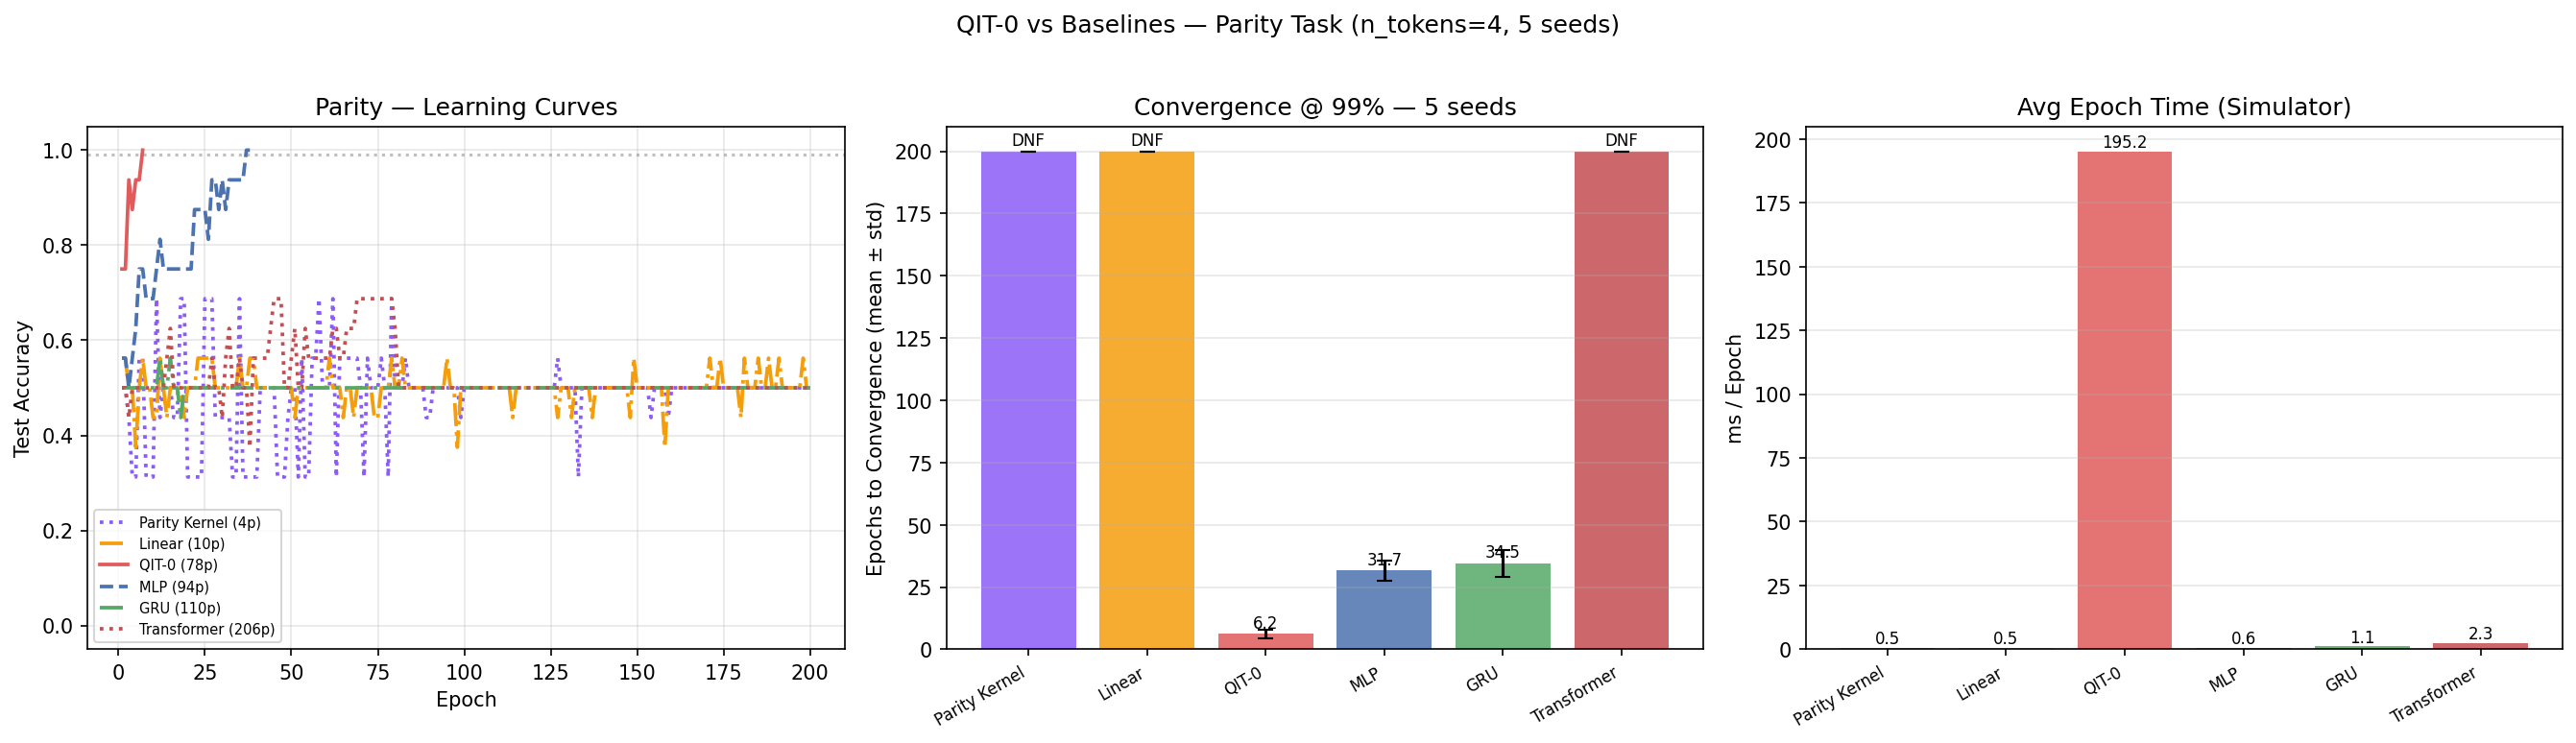
\includegraphics[width=\textwidth]{../results/benchmark_full_parity.png}
\caption{Parity benchmark (5~seeds): test-accuracy learning curves, convergence epoch
         (mean\,$\pm$\,std bars), and wall-clock time per epoch.}
\label{fig:benchmark}
\end{figure}

\subsection{Ablation Study}
\label{sec:ablations}

Table~\ref{tab:ablation} reports convergence for four QIT-0 variants, each with 5 seeds.

\begin{table}[h]
\centering
\caption{Ablation study — entanglement topology. All variants share the same
         78-parameter budget. ``DNF (k/5)'' = $k$ seeds converged.}
\label{tab:ablation}
\begin{tabular}{@{}lll@{}}
\toprule
Variant & Conv.\ Ep.\ (mean$\pm$std) & Conv.\ seeds \\
\midrule
QIT-0 (ring ent., default)     & $6.2\pm1.7$  & 5/5 \\
QIT-0 (star ent.)              & $6.8\pm3.7$  & 5/5 \\
QIT-0 (no ent.)                & $5.0\pm2.1$  & 5/5 \\
QIT-0 (frozen $\Uatt$)         & $22.0\pm9.0$ & 2/5 \\
\bottomrule
\end{tabular}
\end{table}

The ablation results reveal two findings:

\textbf{(1) $\Uent$ is not necessary for parity convergence.} The no-entanglement
variant (5.0\,$\pm$\,2.1 epochs) converges at a rate statistically comparable to the
ring-entanglement default ($6.2\pm1.7$). The star topology performs similarly.
This revises our earlier claim that $\Uent$ is ``critical'': on parity, the learned
$\Uatt$ can distribute correlations from a separable input without a pre-entanglement
step. Whether entanglement is important for tasks with longer-range dependencies
remains to be tested.

\textbf{(2) The learned $\Uatt$ weights are the critical component.} Freezing $\Uatt$
at a random initialisation while allowing only the embedding and decoder to train
reduces convergence reliability to 2/5 seeds and increases mean convergence epoch to
22.0\,$\pm$\,9.0. The learned interference operator is what drives the advantage;
the architecture without training of the quantum layer degrades to a fixed random-feature
classifier.

\begin{figure}[ht]
\centering
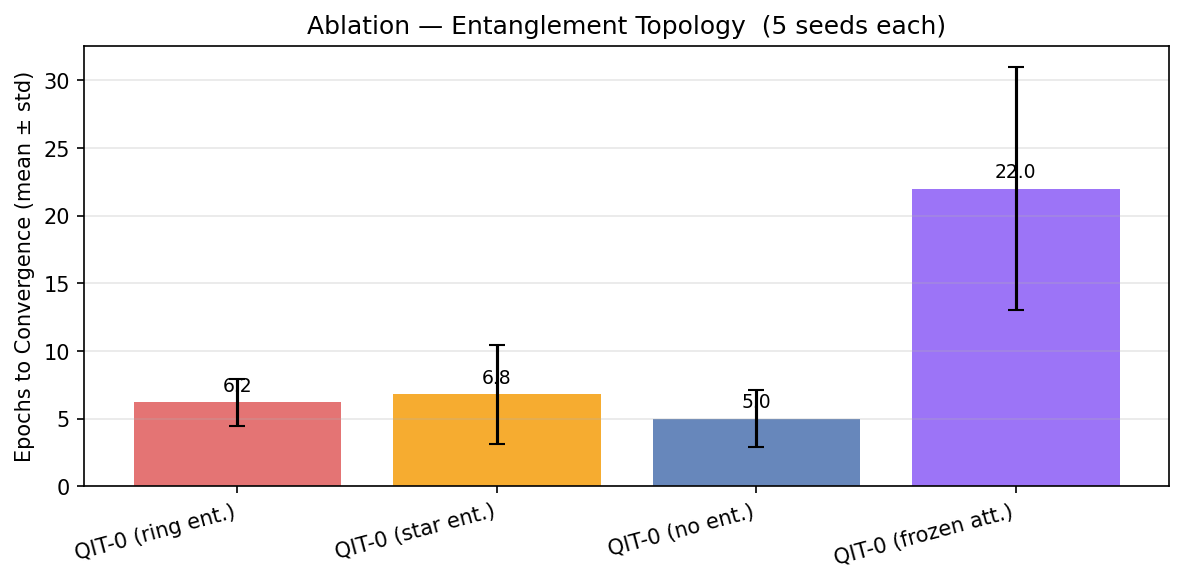
\includegraphics[width=0.65\textwidth]{../results/benchmark_full_ablation.png}
\caption{Ablation: convergence epochs (mean\,$\pm$\,std) for four QIT-0 variants
         on parity (5 seeds each).}
\label{fig:ablation}
\end{figure}

\subsection{Gradient Variance Analysis}
\label{sec:gradvar}

To check for barren plateau pathology~\cite{mcclean2018barren}, we measure the gradient
variance of the loss with respect to $\Uatt$ parameters across 30 random parameter
initialisations at $n_\text{qubits}=8$:

\begin{equation}
  \mathrm{Var}\!\left[\frac{\partial \mathcal{L}}{\partial \theta_i}\right]
  = 3.25\times10^{-4}, \qquad
  \mathbb{E}\!\left[\left|\frac{\partial \mathcal{L}}{\partial \theta_i}\right|\right]
  = 0.013
\end{equation}

The non-zero gradient variance confirms that QIT-0 does not suffer from barren plateaus
at the current 8-qubit scale. Gradient magnitudes are non-negligible and support
parameter-shift-based training. The barren plateau risk at larger scales ($n>16$ qubits)
is a known concern for StronglyEntanglingLayers circuits~\cite{cerezo2023does} and
must be addressed for QIT-1 (\S\ref{sec:future}).

\subsection{First-Token Detection (Negative Control)}
\label{sec:firsttoken}

To test whether QIT's convergence advantage is parity-specific or universal across any
small-input task, we evaluate the same models on \emph{first-token detection}:
predict whether the first token $x_0 = 1$. This task has no global phase structure ---
the answer depends only on one position. Table~\ref{tab:firsttoken} reports results.

\begin{table}[h]
\centering
\caption{First-token detection (5 seeds). A task with positional structure but no
         quantum phase affinity, serving as a negative control.}
\label{tab:firsttoken}
\begin{tabular}{@{}lrll@{}}
\toprule
Model & Params & Conv.\ Ep.\ (mean$\pm$std) & Conv.\ seeds \\
\midrule
\textbf{QIT-0}  & \textbf{78}  & $4.0\pm1.1$ & 5/5 \\
MLP             & 94  & $3.4\pm3.3$ & 5/5 \\
Transformer     & 206 & $5.8\pm1.7$ & 5/5 \\
\bottomrule
\end{tabular}
\end{table}

On first-token detection, QIT-0 ($4.0\pm1.1$) is \emph{not faster} than the MLP
($3.4\pm3.3$) and is comparable to the Transformer ($5.8\pm1.7$). All three models
converge on all 5 seeds. This negative control provides two important clarifications:
(1)~QIT's parity advantage is \textbf{task-specific}, not a universal consequence of
using an expressive circuit on a 16-input dataset; (2)~the convergence advantage on
parity is therefore attributable to the circuit's inductive bias matching the parity
structure, rather than to any generic advantage of quantum circuits over classical models
on small datasets.

\begin{figure}[ht]
\centering
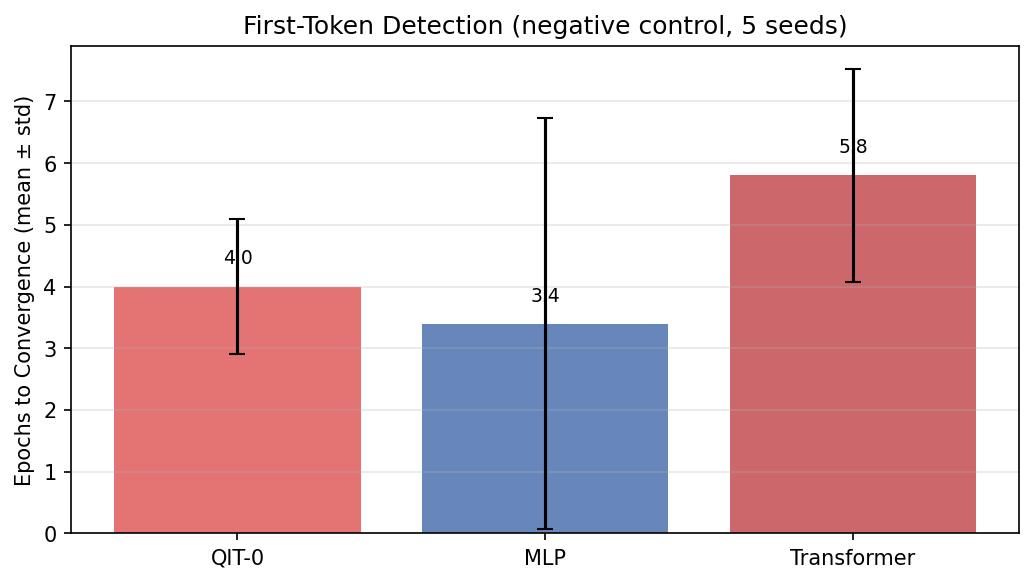
\includegraphics[width=0.55\textwidth]{../results/benchmark_full_firsttoken.png}
\caption{First-token detection (negative control): convergence epoch comparison
         (5 seeds each). QIT-0 is not faster than classical models on this
         positional task with no quantum phase structure.}
\label{fig:firsttoken}
\end{figure}

\subsection{Task Variety: Parity Scaling and Structural Generality}
\label{sec:taskvariety}

Having established QIT-0's advantage on 4-bit parity and its absence on first-token
detection, we ask two further questions: (1)~does the advantage scale gracefully with
parity degree, or is 4-bit an artefact? (2)~does QIT's inductive bias extend beyond
global parity to other XOR-structured tasks?

We evaluate five tasks under the same 5-seed memorisation protocol (all 16 inputs):
\textbf{2-bit partial parity} ($x_0 \oplus x_1$),
\textbf{3-bit partial parity} ($x_0 \oplus x_1 \oplus x_2$),
\textbf{4-bit full parity} (main benchmark),
\textbf{first-token detection} (positional negative control), and
\textbf{palindrome detection} (predict whether $\mathbf{x} = \text{reverse}(\mathbf{x})$).
Palindromes are 4/16 of all inputs, giving a 75\% majority-class baseline.
Table~\ref{tab:taskvariety} reports convergence epochs.

\begin{table}[h]
\centering
\caption{Task variety benchmark (5 seeds each). Convergence $\ge99\%$ test accuracy.
         ``Conv/5'' = number of seeds that converged within the epoch limit.}
\label{tab:taskvariety}
\begin{tabular}{@{}lrll@{}}
\toprule
Model & Params & Conv.\ Ep.\ (mean$\pm$std) & Conv/5 \\
\midrule
\multicolumn{4}{@{}l}{\textit{2-bit partial parity ($x_0\oplus x_1$)}} \\[1pt]
\quad\textbf{QIT-0}  & \textbf{78} & $\mathbf{4.6\pm1.0}$ & 5/5 \\
\quad MLP            & 94          & $8.6\pm7.9$           & 5/5 \\
\quad Transformer    & 206         & $28.0\pm9.1$          & 5/5 \\
\midrule
\multicolumn{4}{@{}l}{\textit{3-bit partial parity ($x_0\oplus x_1\oplus x_2$)}} \\[1pt]
\quad\textbf{QIT-0}  & \textbf{78} & $\mathbf{5.0\pm2.2}$ & 5/5 \\
\quad MLP            & 94          & $23.8\pm9.0$          & 4/5 \\
\quad Transformer    & 206         & $25.3\pm7.3$          & 3/5 \\
\midrule
\multicolumn{4}{@{}l}{\textit{4-bit full parity ($x_0\oplus x_1\oplus x_2\oplus x_3$)}} \\[1pt]
\quad\textbf{QIT-0}  & \textbf{78} & $\mathbf{6.2\pm1.7}$ & 5/5 \\
\quad MLP            & 94          & $31.7\pm4.1$          & 3/5 \\
\quad Transformer    & 206         & DNF                   & 0/5 \\
\midrule
\multicolumn{4}{@{}l}{\textit{First-token detection ($x_0$) --- negative control}} \\[1pt]
\quad\textbf{QIT-0}  & \textbf{78} & $4.0\pm1.1$ & 5/5 \\
\quad MLP            & 94          & $3.4\pm3.3$ & 5/5 \\
\quad Transformer    & 206         & $5.8\pm1.7$ & 5/5 \\
\midrule
\multicolumn{4}{@{}l}{\textit{Palindrome detection ($\mathbf{x} = \mathrm{rev}(\mathbf{x})$)}} \\[1pt]
\quad\textbf{QIT-0}  & \textbf{78} & $\mathbf{13.2\pm3.2}$ & 5/5 \\
\quad MLP            & 94          & $53.4\pm54.5$          & 5/5 \\
\quad Transformer    & 206         & $55.0\pm0.0$           & 1/5 \\
\bottomrule
\end{tabular}
\end{table}

\textbf{Parity scaling.}
QIT-0 scales monotonically with parity degree: $4.6\pm1.0$ epochs (2-bit),
$5.0\pm2.2$ (3-bit), $6.2\pm1.7$ (4-bit), with 5/5 seeds converging throughout.
The increment per additional XOR input is small ($\sim$0.8 epochs/bit).
Classical models degrade sharply: MLP drops from 5/5 converging seeds (2-bit)
to 3/5 (4-bit) while its mean epoch count quadruples; the Transformer drops from
5/5 seeds at 28 epochs to 0/5 seeds on 4-bit parity.
The monotonicity of QIT-0 across parity degrees indicates that the $\mathbb{F}_2$-structured
inductive bias is not an artefact of the specific 4-bit setting.

\textbf{Palindrome detection.}
Palindrome detection requires $(x_0 = x_3) \wedge (x_1 = x_2)$, which is logically
equivalent to $(x_0 \oplus x_3 = 0) \wedge (x_1 \oplus x_2 = 0)$
--- a conjunction of position-pair XOR checks.
QIT-0 converges in $13.2\pm3.2$ epochs (5/5 seeds), substantially faster than
MLP ($53.4\pm54.5$, 5/5 seeds but extremely high variance) and Transformer (55 epochs,
1/5 seeds only).
The 13.2-epoch cost is roughly twice the 4-bit parity cost (6.2 epochs), consistent
with palindrome requiring two independent XOR conditions to be satisfied simultaneously.
This result extends QIT's advantage to tasks with XOR-like relational structure even
when those comparisons involve specific position pairs rather than all tokens globally.

\textbf{When does the advantage not appear?}
First-token detection (Table~\ref{tab:firsttoken}) shows no QIT advantage: all three
models converge at similar rates ($\approx$3--6 epochs, 5/5 seeds). The contrast is
clear: tasks with $\mathbb{F}_2$-structured relational checks favour QIT; tasks that
depend on a single token's value do not.

\begin{figure}[ht]
\centering
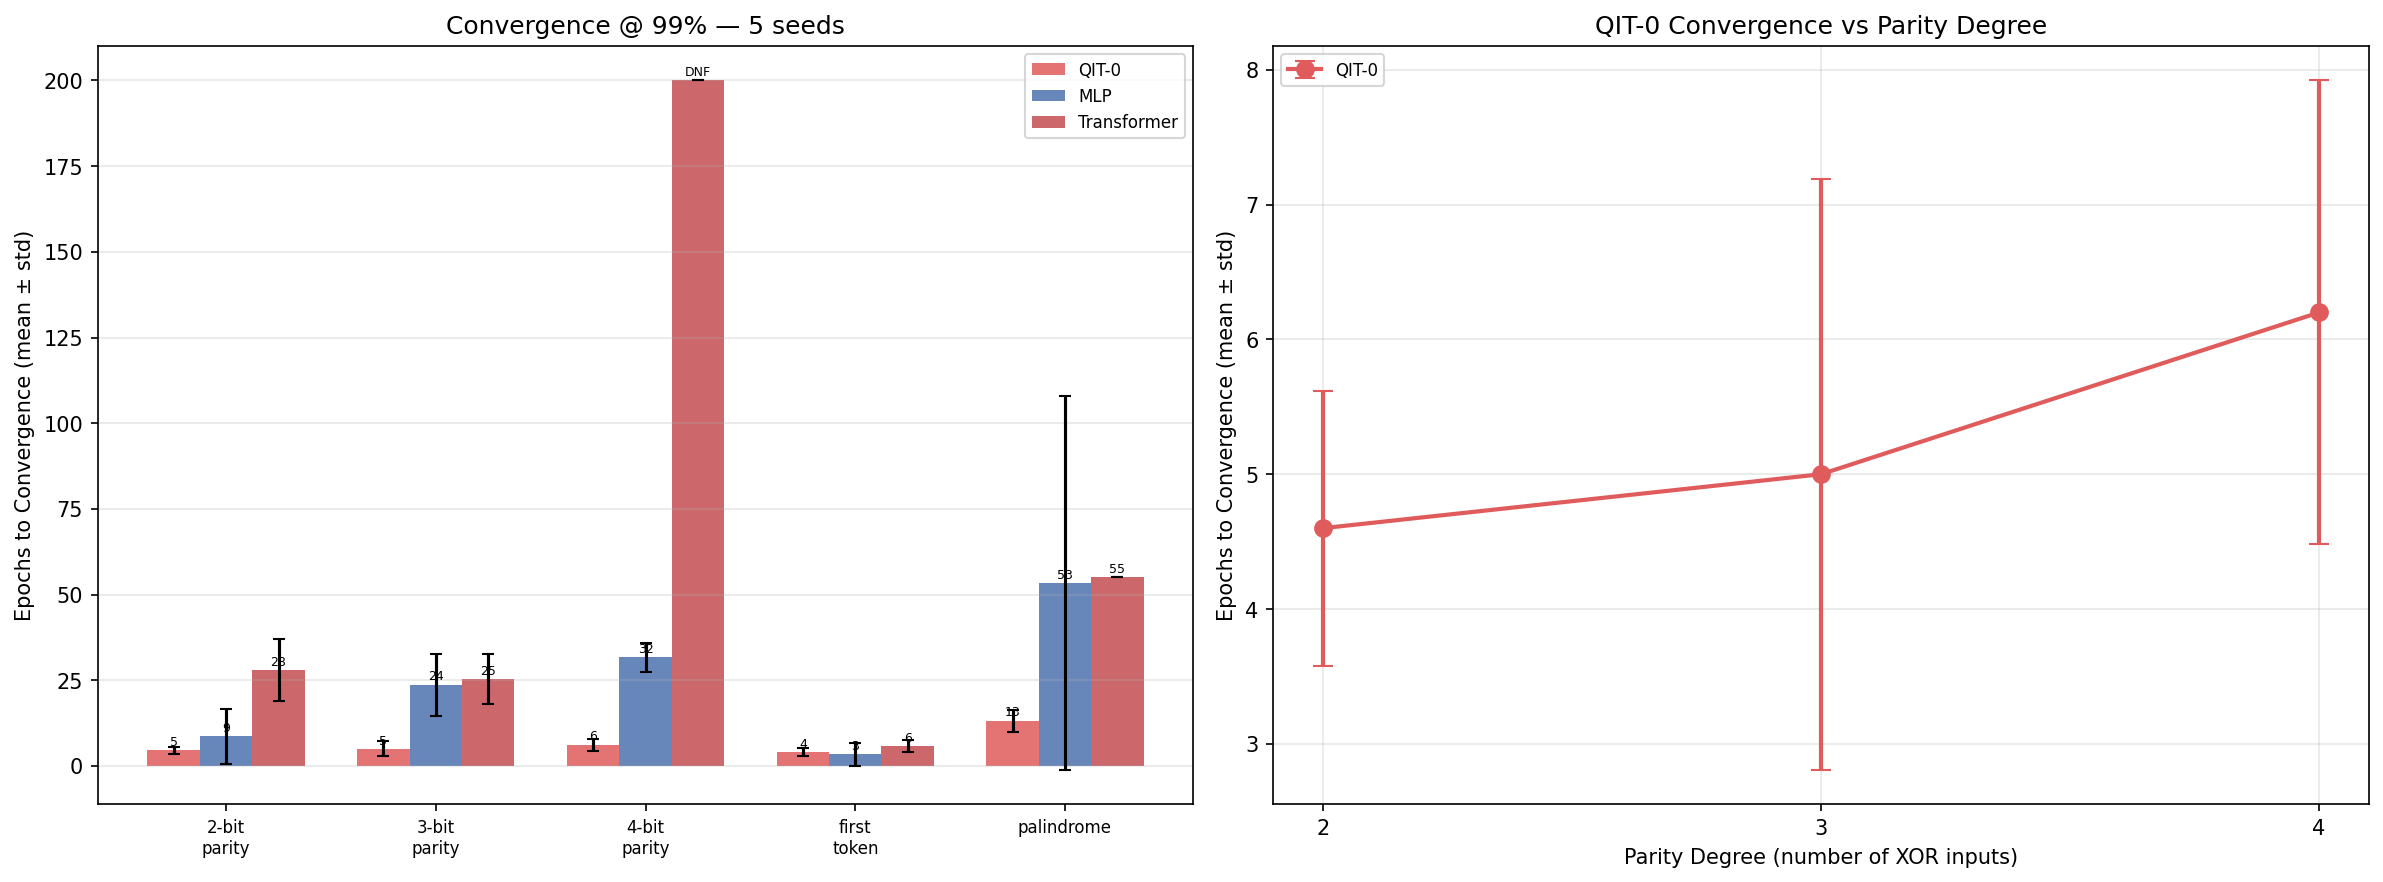
\includegraphics[width=0.75\textwidth]{../results/benchmark_tasks.png}
\caption{Task variety benchmark (5 seeds). \textit{Left}: convergence epoch by task
         and model (DNF shown at epoch limit). \textit{Right}: QIT-0 parity-degree
         scaling --- a monotonic, graceful increase from $4.6\pm1.0$ (2-bit) to
         $6.2\pm1.7$ (4-bit).}
\label{fig:taskvariety}
\end{figure}

%% ─────────────────────────────────────────────────────────────────────────────
\section{Discussion}
\label{sec:discussion}

\subsection{Why Does QIT Converge So Fast on Parity?}

The parity function $y = x_1 \oplus x_2 \oplus \cdots \oplus x_n$ is a linear function
over $\Ftwo$. This maps cleanly to quantum phase arithmetic. Consider encoding each bit
$x_i \in \{0,1\}$ as a phase kick: the operator $Z^{x_i}$ maps $\ket{+} \to (-1)^{x_i}\ket{+}$.
After $n$ such kicks the phase accumulated is $(-1)^{x_1 \oplus \cdots \oplus x_n}$ ---
directly encoding the parity bit as a global phase. This is the mechanism exploited by the
Bernstein-Vazirani~\cite{bernstein1997quantum} algorithm to determine a hidden linear
Boolean function in a \emph{single} quantum query.

QIT's angle encoding does not apply this operator exactly, but it produces an analogous
effect: $RY(\phi_{t,j})$ rotates qubit $(t,j)$ toward $\ket{1}$ proportionally to the
token's embedding value. After the ring entanglement step $\Uent$, each qubit's state
depends on its neighbours, creating a distributed phase representation of the full input
sequence. The learned $\Uatt(\theta_\text{attn})$ must then find the unitary that
projects even-parity configurations onto one amplitude pattern and odd-parity
configurations onto another.

Because parity is a degree-1 polynomial over $\Ftwo$ (hence the lowest-complexity
nontrivial Boolean function), this projection requires relatively few parameters: the
interference pattern is simple. The $6.2\pm1.7$~epoch convergence (all 5 seeds) is
consistent with the circuit starting near the correct basin of attraction under random
initialisation --- the \texttt{StronglyEntanglingLayers} circuit is expressive enough to
represent the parity unitary, and gradient descent finds it reliably.

The ablation (Table~\ref{tab:ablation}) shows that $\Uent$ is not necessary: the
no-entanglement variant ($5.0\pm2.1$ epochs) converges at a comparable rate.
The learned $\Uatt$ can spread correlations from a separable input on its own for
parity. The critical architectural component is the \emph{trained} interference operator,
not the pre-entanglement step. This refines our understanding: the inductive bias comes
from the expressive, trainable quantum circuit, not from the specific initialisation
of cross-token entanglement.

Classical Transformers do not exploit this structure. Dot-product attention scores
$\exp(q_i \cdot k_j / \sqrt{d})$ are symmetric bilinear functions of token pairs,
with no algebraic relationship to $\Ftwo$ arithmetic. The model must discover the parity
function by composing pairwise interactions --- and in our multi-seed experiment, it
\emph{fails to do so reliably}: 0/5 seeds converge in 200~epochs.

\subsection{Limitations of QIT-0}

\textbf{Memorisation, not generalisation.} The task has 16 inputs and the training set
contains all of them. We measure whether the model can encode a specific boolean function,
not whether it generalises to unseen inputs. This is an appropriate first test for a
new architecture but should not be conflated with claims about generalisation.

\textbf{Simulation overhead is real.} The $\approx195$~ms/epoch cost means QIT-0 is not
practically useful on a classical computer for tasks where a classical model suffices.
The value proposition of QIT depends on either (a)~tasks where sample efficiency is so
high that total wall-clock time is competitive despite per-step overhead, or (b)~access
to quantum hardware where circuit execution is fast.

\textbf{Parity is permutation-invariant.} As noted in \S\ref{sec:firsttoken}, the
advantage on parity is task-specific: QIT is not faster than MLP on first-token
detection (which has no global phase structure). The parity advantage reflects inductive
bias for $\Ftwo$-structured functions, not a universal superiority of quantum circuits
on small datasets.

\textbf{Limited task breadth.} Results cover five structured tasks on 4-token binary
sequences. Across these tasks, QIT-0 is fast on $\mathbb{F}_2$-structured functions
(parity variants, palindrome) and at par with classical on purely positional tasks
(first-token). Whether this advantage extends to longer sequences, higher-degree Boolean
functions, continuous-valued inputs, or natural-language tasks remains unknown.

\textbf{Simulator fidelity.} PennyLane's \texttt{default.qubit} computes exact
statevector evolution with no noise. Real quantum devices have gate errors, decoherence,
and measurement noise. Performance on real hardware \planned{} may differ substantially.

\subsection{What This Work Claims and Does Not Claim}

\textbf{Claims:}
\begin{itemize}
  \item Interference-based attention is a viable architectural concept: a quantum circuit
        can serve as a learned attention operator and achieve competitive performance on
        structured tasks.
  \item QIT-0 is sample-efficient on parity: $6.2\pm1.7$ epochs (5/5 seeds converging)
        vs.\ 31.7--34.5 epochs for the two classical models that converge at all
        (MLP: 3/5 seeds, GRU: 2/5 seeds), with the Transformer failing entirely.
  \item The inductive bias matches $\mathbb{F}_2$-structured tasks: QIT-0 is faster
        on all parity variants (2-, 3-, and 4-bit) and on palindrome detection (which
        decomposes into position-pair XOR checks). Purely positional tasks (first-token
        detection) show no QIT advantage.
  \item The parity advantage scales gracefully: QIT-0 adds $\approx$0.8 epochs per
        additional XOR input (4.6$\to$5.0$\to$6.2 epochs, 2$\to$3$\to$4 bits),
        while classical models degrade sharply.
  \item The learned $\Uatt$ is the key component; pre-entanglement ($\Uent$) is helpful
        but not strictly necessary for parity.
\end{itemize}

\textbf{Does not claim:}
\begin{itemize}
  \item Quantum machine learning is generally superior to classical machine learning.
  \item QIT-0 is practically deployable.
  \item The observed sample efficiency advantage generalises to arbitrary tasks.
  \item The wall-clock advantage is positive at application scales.
\end{itemize}

%% ─────────────────────────────────────────────────────────────────────────────
\section{Future Work}
\label{sec:future}

\subsection{QIT-1: Larger Circuits \planned{}}

The natural next step is scaling the circuit to longer sequences and deeper architectures.
QIT-1 is planned with $n_\text{tokens} \in \{6, 8\}$ and
$n_\text{qubits\_per\_token} \in \{3, 4\}$, giving circuits of 18--32 qubits. This will
test whether the sample efficiency advantage persists as sequence length grows and whether
qubit count scaling is favourable compared to classical attention's $O(n^2)$ scaling.

\subsection{Ablation Studies}
\label{sec:ablations_future}

The entanglement topology and frozen-attention ablations are completed and reported in
\S\ref{sec:ablations}. Remaining open ablations:

\begin{itemize}
  \item \textbf{Encoding strategy.} QIT-0 uses angle ($RY$) encoding. Amplitude,
        basis, and phase encodings are implemented in \texttt{qit/encoding/} but not
        yet benchmarked.

  \item \textbf{Number of attention layers.} QIT-0 uses $n_\text{layers} = 2$ for
        $\Uatt$. How does convergence speed and gradient trainability scale with circuit depth?

  \item \textbf{Linear CNOT topology.} The ring and star topologies are evaluated;
        a linear (chain) topology is a natural next comparison.
\end{itemize}

\subsection{Tasks Beyond Parity}

The task-variety benchmark (\S\ref{sec:taskvariety}) establishes that QIT's advantage
extends to partial parity variants and palindrome detection. Remaining planned evaluations:
\textbf{binary arithmetic} (carry propagation as a structured $\mathbb{F}_2$ task),
\textbf{balanced parentheses} (formal language with long-range dependency), and
\textbf{continuous-valued inputs} (breaking the angle-encoding specialisation).
In particular, the linear CNOT chain topology (not yet benchmarked) may exhibit
different parity-scaling behaviour compared to ring and star topologies already evaluated.

\subsection{Interference Visualisation \planned{}}

Planned visualisations include: Bloch sphere trajectories for individual qubits as
input changes; amplitude probability distributions $|\langle x | \Psi \rangle|^2$ as a
function of input parity; and mutual information between token-register subsystems
before and after $\Uent$.

\subsection{Real Hardware Evaluation \planned{}}

Evaluating QIT-0 on real hardware --- IBM~Q via Qiskit or Quantinuum via TKET ---
is essential for assessing practical viability. Key questions: How much does gate noise
degrade accuracy at $n_\text{qubits} = 8$? Does the learned circuit require error
mitigation? What is the actual runtime on current NISQ hardware~\cite{preskill2018quantum}?

\subsection{Scaling Laws \planned{}}

Classical Transformers exhibit power-law scaling in loss as a function of parameter count
and data volume. Whether a similar relationship holds for QIT --- and whether the exponent
is more favourable than for classical attention --- is an empirical question requiring
systematic experiments across circuit sizes, sequence lengths, and task complexities.

%% ─────────────────────────────────────────────────────────────────────────────
\section{Conclusion}
\label{sec:conclusion}

We have introduced QIT-0, the first prototype of the Quantum Interference Transformer:
a sequence model in which token relationships are resolved by amplitude interference in a
parameterised quantum circuit rather than by explicit dot-product attention scores.

On the 4-bit parity memorisation benchmark, QIT-0 achieves 100\% accuracy in
$\mathbf{6.2\pm1.7}$ \textbf{epochs} with \textbf{78 parameters}, converging reliably on
all 5 random seeds. In contrast, MLP converges on 3/5 seeds (31.7\,$\pm$\,4.1 epochs),
GRU on 2/5 seeds (34.5\,$\pm$\,5.5 epochs), and the Transformer on 0/5 seeds in 200~epochs.
An ablation confirms that the learned interference operator $\Uatt$ is the key driver;
pre-entanglement ($\Uent$) is helpful but not strictly required for this task.

A five-task variety experiment (\S\ref{sec:taskvariety}) strengthens the picture.
On $\mathbb{F}_2$-structured tasks, QIT-0 is consistently fast: partial parity
scales gracefully (4.6$\pm$1.0 epochs at 2-bit, 5.0$\pm$2.2 at 3-bit, 6.2$\pm$1.7 at
4-bit, all 5/5 seeds), and palindrome detection (a conjunction of position-pair XOR
checks) converges in 13.2$\pm$3.2 epochs versus 53 for MLP and DNF for the Transformer.
On a purely positional task (first-token detection), QIT-0 is \emph{not} faster than
classical models --- confirming the advantage is structurally specific, not universal.

The result supports the core claim: \emph{for tasks whose structure maps naturally to
quantum phase dynamics, interference-based attention exhibits strong inductive bias and
superior sample efficiency}. We are careful not to over-interpret this: QIT-0 is a
prototype on a small set of structured tasks, running on a quantum simulator with
substantial wall-clock overhead. The practical case for QIT depends on future work with
larger circuits, more diverse tasks, and real quantum hardware.

The code for QIT-0 --- including the circuit, training harness, baselines, ablations,
and benchmark --- is fully implemented and publicly available at
\url{https://github.com/madmishu007/qit}. Encoding strategies, entanglement topologies,
and attention circuit designs can be swapped independently via configuration flags,
providing a modular platform for systematic experimentation as the field of quantum
sequence modelling matures.

\bigskip
\noindent\textit{Interference computes. The question is: what else can it learn?}

%% ─────────────────────────────────────────────────────────────────────────────
\bibliographystyle{plainnat}
\bibliography{references}

%% ─────────────────────────────────────────────────────────────────────────────
\section*{Generative AI Disclosure}

During the preparation of this work, I used ChatGPT (OpenAI) and Claude (Anthropic) for grammar and language editing, and for code generation assistance. All research, methodology, analysis, results, and conclusions are my own. I reviewed all AI-assisted content and take full responsibility for the work.

%% ─────────────────────────────────────────────────────────────────────────────
\appendix

\section{QIT-0 Configuration Summary}
\label{app:config}

\begin{lstlisting}
Model:       QIT-0
Task:        4-bit binary parity (memorisation, all 16 inputs)
Backend:     PennyLane default.qubit (statevector simulator)
Platform:    Apple Silicon, macOS 25.3, PyTorch 2.12,
             PennyLane 0.45, Python 3.11

Architecture:
  vocab_size          = 2
  n_tokens            = 4
  n_qubits_per_token  = 2
  n_qubits (total)    = 8
  n_layers            = 2
  entangle_topology   = "ring"  # also: "star", "none"

  Embedding:    nn.Embedding(2, 2)                       -> 4 params
  Encoding:     RY(tanh(e) * pi) per qubit
  Entanglement: Ring CNOT (4 tokens, circular)
  Attention:    StronglyEntanglingLayers(n_layers=2, n_qubits=8) -> 48 params
  Mix:          BasicEntanglerLayers(n_layers=1, n_qubits=8)     ->  8 params
  Measurement:  <Z_i> for i in {0,...,7}
  Decoder:      nn.Linear(8, 2)                          -> 18 params
  Total params: 78

Training (multi-seed protocol):
  Optimizer:  Adam, lr = 0.05
  Loss:       CrossEntropyLoss
  Batch size: 8
  Seeds:      5 (independent model init + data shuffle)
  Conv. ep.:  6.2 +/- 1.7 (mean +/- std, all 5 seeds converge)
  Grad steps: 12.4 (mean; 2 steps/epoch at batch_size=8)
\end{lstlisting}

\section{Baseline Architecture Summaries}
\label{app:baselines}

\textbf{MLP (94 parameters)}
\begin{lstlisting}
nn.Embedding(2, 2) -> flatten -> nn.Linear(8, 8) -> ReLU -> nn.Linear(8, 2)
\end{lstlisting}

\textbf{GRU (110 parameters)}
\begin{lstlisting}
nn.Embedding(2, 2) -> GRU(input=2, hidden=4) -> last hidden -> nn.Linear(4, 2)
\end{lstlisting}

\textbf{Transformer (206 parameters)}
\begin{lstlisting}
nn.Embedding(2, 4) + positional encoding ->
TransformerEncoderLayer(d_model=4, nhead=2, dim_feedforward=8) ->
mean pooling -> nn.Linear(4, 2)
\end{lstlisting}

All baselines: Adam, $\eta = 0.05$, CrossEntropyLoss, batch size 8.

\end{document}
